\section{Churn de usuarios en Spotify}

% ---------------------------------------------------------------------------------------------------------- %

\subsection{Descripción del proyecto}

\subsubsection{Objetivo}

El objetivo es predecir la pérdida de usuarios (\textit{churn} en inglés) en función de datos personales de los usuarios y de su interacción con el servicio. Las conclusiones de este análisis intentan ayudar en la toma de decisiones de la empresa para reducir el número de cancelaciones.

\subsubsection{Datos}

El conjunto de datos que usamos para entrenar nuestro modelo está disponible en la base de datos de Kaggle: \href{https://www.kaggle.com/datasets/nabihazahid/spotify-dataset-for-churn-analysis/data}{Spotify Analysis Dataset 2025}. 
Ya hemos descargado el fichero con extensión \texttt{.csv} en el directorio \texttt{datasets}.

En el \textit{dataset} encontramos 12 columnas, donde diferenciamos a los atributos de la variable objetivo. 
La variable objetivo, o \textit{target}, es aquella que deseamos predecir a partir de los atributos; 
en este caso esta es \code{is\_churned}, y es una variable binaria que toma dos valores:
\begin{itemize}
    \item \code{1}, cuando el usuario ha cancelado su cuenta; o
    \item \code{0}, cuando el usuario sigue activo.
\end{itemize}

En los atributos podemos diferenciar dos principales tipos de variables: numéricas y categóricas. 
Dentro de las variables numéricas, se pueden distinguir aquellas representadas como números enteros y las que se expresan en formato en coma flotante.

Cada tipo de dato requiere un tratamiento específico, y algunos modelos serán más adecuados que otros para cada tipo. En ocasiones, será necesario modificar la codificación para garantizar una mejor compatibilidad con el modelo.
\begin{itemize}
    \item Modelos como los de árboles de decisión, \textit{Random Forest} o \textit{Naive Bayes} ---en su forma base--- funcionan con datos categóricos.
    \item Modelos como los de \textit{K-Nearest Neighbour}, las \textit{Support Vector Machine} o las redes neuronales, ---de nuevo, hablamos en su forma base--- trabajan con datos numéricos.
\end{itemize}

Además, las variables categóricas y numéricas presentan una semántica muy distinta. Generalmente, las variables categóricas no presentan un orden inherente en sus valores, a diferencia de las variables numéricas. Sin embargo, es común encontrar en ciertos conjuntos de datos variables codificadas con números enteros que actúan como códigos, pero que, desde un punto de vista semántico, se comportan como variables categóricas, ya que no presentan un orden inherente en sus valores; por ejemplo, el código \code{2} no está más cerca del \code{3} que del \code{4}. Cuando identifiquemos este tipo de variables, el primer paso en el preprocesamiento será cambiar su codificación para evitar que los modelos los interpreten como variables numéricas, que puedan llegar a tener alterar el sentido de una predicción.

El caso opuesto también puede darse cuando encontramos variables categóricas que presentan un orden lineal en su significado, aunque este no esté reflejado en su valor de texto. 
A estas variables, les asignaremos valores numéricos para capturar ese orden en el análisis.

En este proyecto, encontramos una variable de tipo categórico representada por números enteros, esta es la variable objetivo \code{is\_churned}, anteriormente analizada. 
En la primera modificación del conjunto de datos original, cambiaremos el tipo de dato de esta columna a \textit{string}, reemplazando el valor \code{1} por \code{CHURNED}, y el \code{0} por \code{NOT\_CHURNED}.

El resto de variables del dataset son las siguientes:

    \begin{itemize}
        \item \code{user\_id}:
        \item \code{gender}: De tipo categórico (\textit{string}). Genéro del usuario.
        \item \code{age}: De tipo entero. Edad del usuario.
        \item \code{country}: De tipo categórico (\textit{string}). País del usuario. 
        \item \code{subscription\_type}: De tipo categórico (\textit{string}). Tipo de suscripción del usuario.
        \item \code{listening\_time}: De tipo entero. Número de minutos por día reproduciendo, en poromedio. 
        \item \code{songs\_played\_per\_day}: De tipo entero. Número de canciones reproducidas diariamente, en promedio.
        \item \code{skip\_rate}: De tipo decimal (\textit{float}). Porcentaje de canciones saltadas. 
        \item \code{device\_type}: De tipo categórico (\textit{string}). Tipo de dispositivo usado. 
        \item \code{ads\_listened\_per\_week}: De tipo entero. Número de anuncios reproducidos por semana.
        \item \code{offline\_listening}: De tipo entero, aunque semánticamente booleano. Uso del modo \textit{offline}. 
    \end{itemize}

% ---------------------------------------------------------------------------------------------------------- %

\subsection{Exploración, visualización y preprocesado de datos}

\subsubsection{Carga de datos}

La carga de datos la realizamos con un nodo de entrada <<CSV Reader>>.

\begin{figure}[h!]
    \fbox{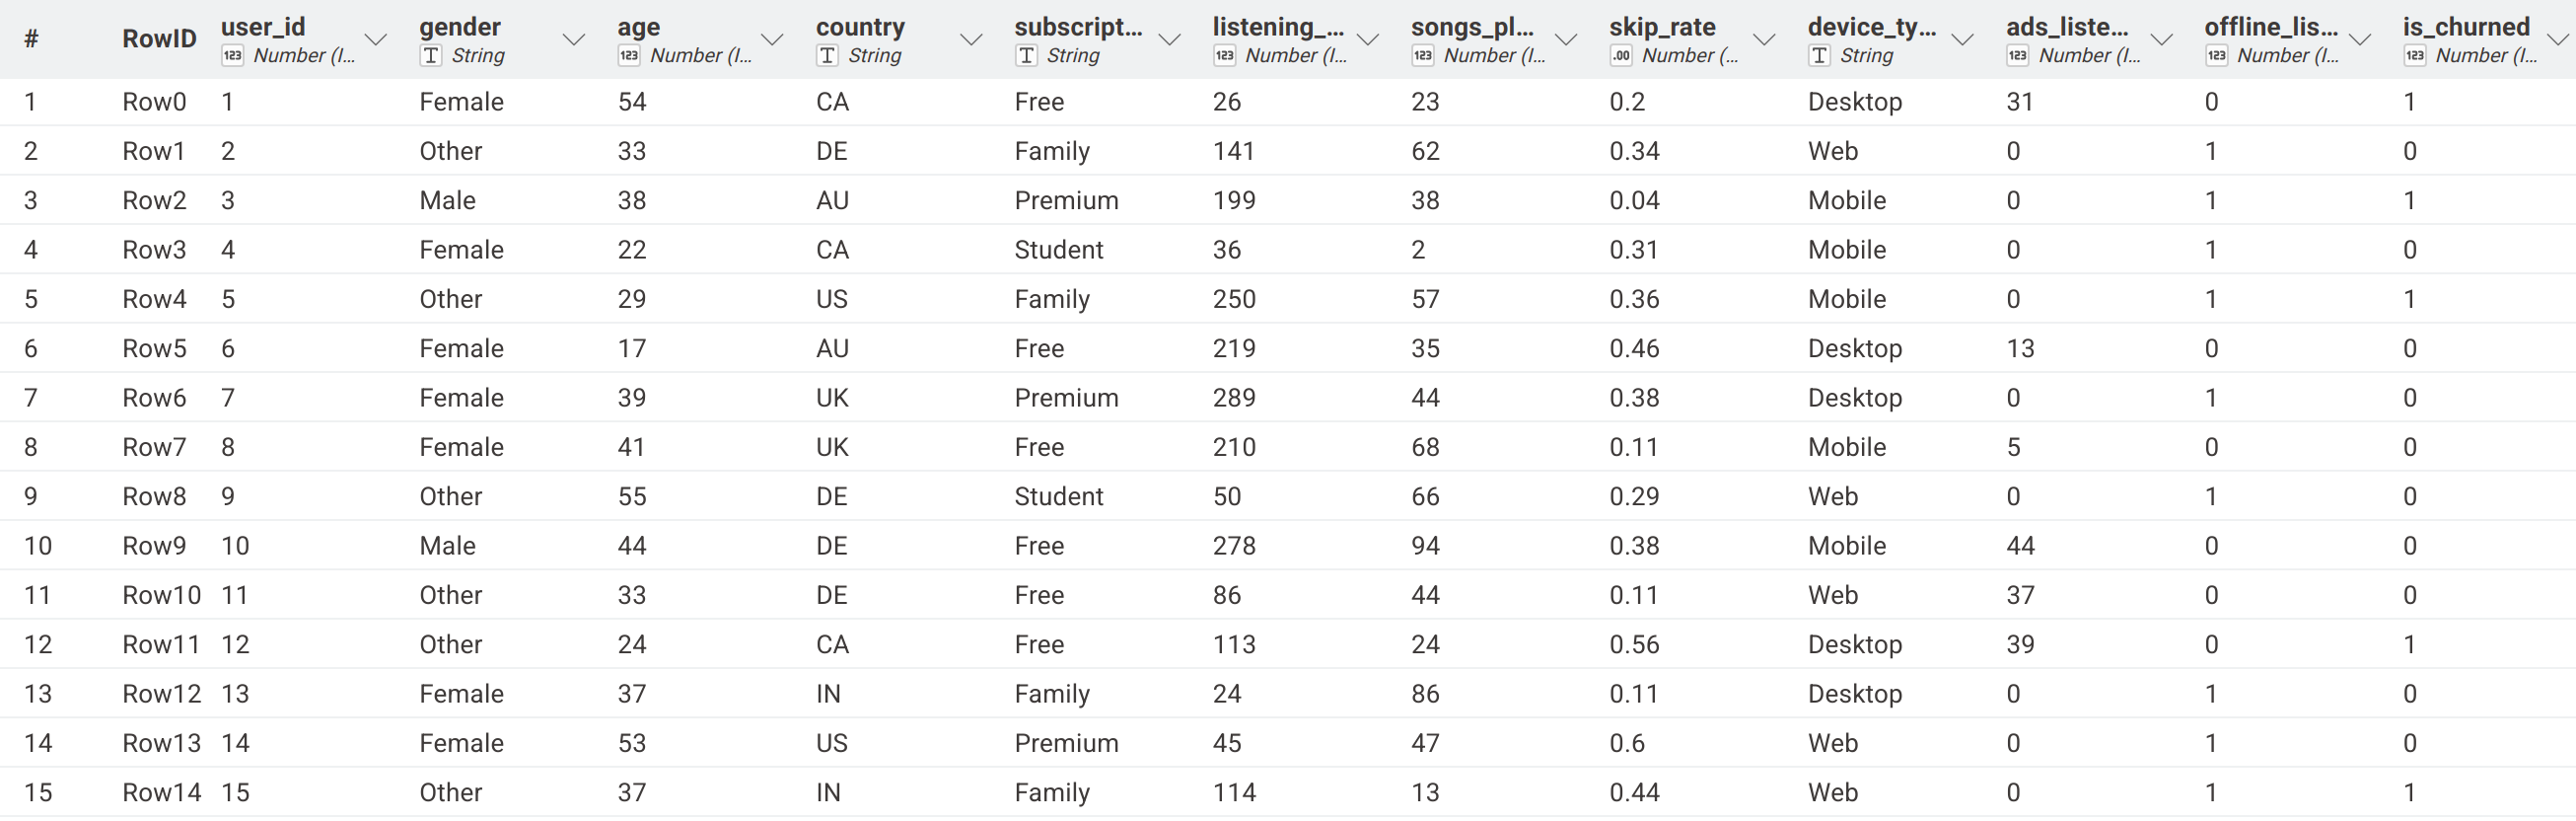
\includegraphics[width=1.0\textwidth, keepaspectratio]{secciones/sec2/imagenes/churn_spotify_CSV_Reader.png}}
    \caption{
        Visualización de los datos crudos (\textit{raw data}, en inglés) del primer problema
    }
    \label{fig:spotify_churn_CSVReader_RawData}
\end{figure}

En la Figura \ref{fig:spotify_churn_CSVReader_RawData} vemos que el conjunto de datos tiene 8 000 instancias, cada con 12 características y su etiqueta ---que es como se denomina al valor real de la variable \textit{target} en cada instancia---.

En las siguientes subsecciones limpiaremos y prepararemos los datos, para facilitar su interpretación y exploración inicial. Y es que, muchas veces, los datos pueden estar incompletos, contener valores atípicos o estar en formatos difíciles de analizar directamente. Posteriormente, realizaremos ajustes específicos en función de los requisitos de cada modelo.

\subsubsection{Análisis de variables}

Ahora realizaremos un pequeño análisis tanto de las características como de la variable objetivo. Comenzaremos utilizando el nodo <<Data Explorer>> de la extensión \textit{KNIME JavaScript Views (Labs)}.

\paragraph*{Variables categóricas.}

La variable objetivo ha sido convertida a una variable categórica (\code{churned\_status}), para poder analizarse como tal. En la Figura \ref{fig:spotify_churn_Statistics_Nominal_Attributes} podemos ver los resultados del análisis exploratorio sobre cada variable categórica. 

\begin{figure}[h!]
    \fbox{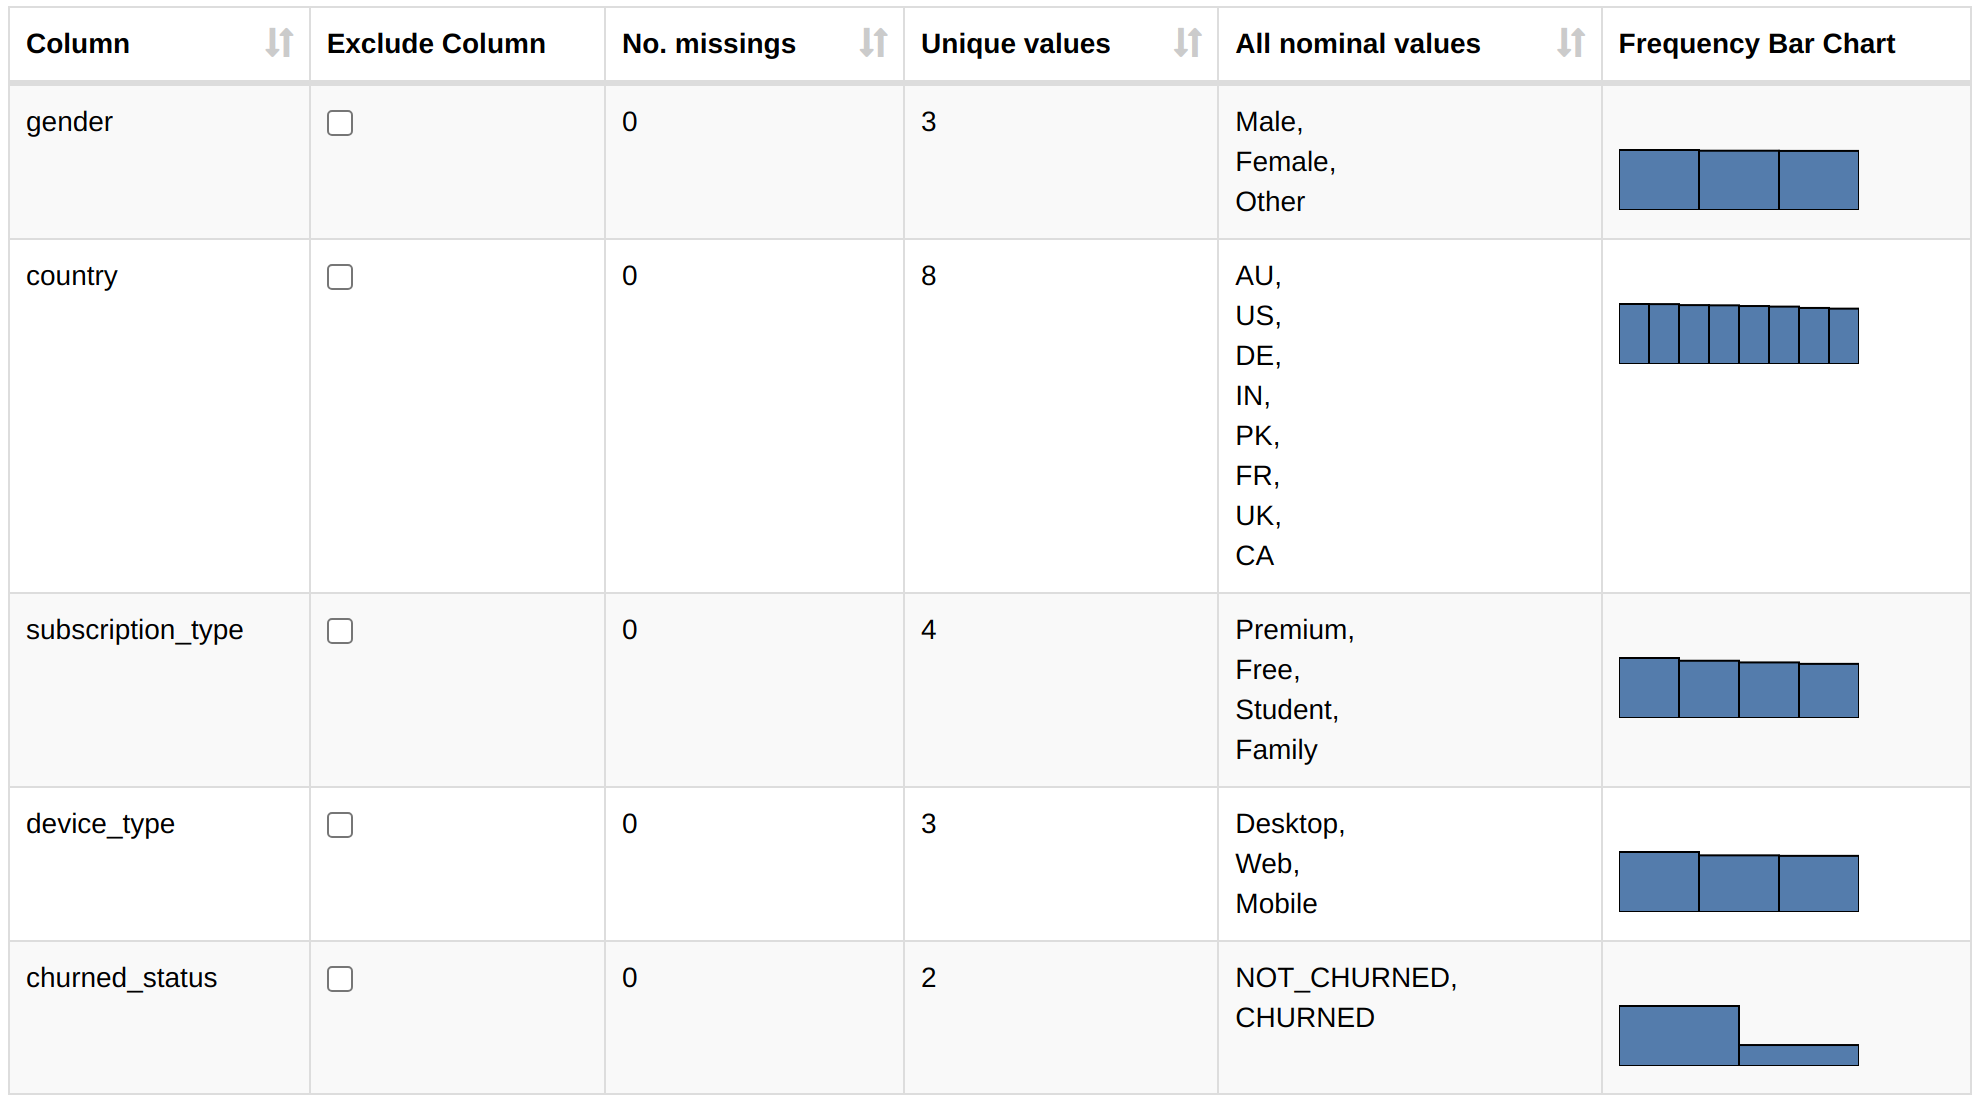
\includegraphics[width=1.0\textwidth, keepaspectratio]{secciones/sec2/imagenes/churn_spotify_statistical_nominal_attributes.png}}
    \caption{Visualización del análisis exploratorio de variables categóricas.}
    \label{fig:spotify_churn_Statistics_Nominal_Attributes}
\end{figure}

Analicemos la información extraída de este reporte:

\begin{itemize}
    \item \code{gender} tiene tres valores posibles: \code{Male}, \code{Female} y \code{Other}. La frecuencia de los tres grupos es aparentemente idéntica. 
    
    \item \code{country} tiene ocho valores posibles: \code{AU} (Australia), \code{US} (Estados Unidos), \code{DE} (Dinamarca), \code{IN} (India), \code{PK} (Pakistán), \code{FR} (Francia), \code{UK} (Reino Unido) y \code{CA} (Canadá). La frecuencia de todos los grupos es muy similar, 
    
    \item \code{subscription\_type} tiene cuatro valores posibles: \code{Free}, \code{Premium}, \code{Student} y \code{Family}. 
    
    \item \code{device\_type} tiene tres valores posibles: \code{Desktop}, \code{Web} y \code{Mobile}. 

\end{itemize}

En todas las características comprobamos que las diversas categorías están muy equilibradas. La mayor diferencia de ocurrencias entre dos categorías de cada variable son de apenas un 0.5\% en \code{gender}, 1\% en \code{country}, 2.4\% en \code{subscription\_type} y 2.3\% en \code{device\_type}. La variable objetivo sí presenta dos clases desbalanceadas: un 74\% de las instancias son de usuarios que no han cancelado su cuenta, dejando solo un 26\% de las instancias positivas. 

¿Cómo se relacionan entre ellas? En la Figura \ref{fig:churn_spotify_ParallelCategories_NominalAttributes} se muestra cómo se corresponden estas variables categóricas en sus distintos valores con las clases de la variable objetivo mediante un gráfico de Categorías Paralelas. Este gráfico es súmamente útil, ya que nos permite ver qué proporción de cada valor hay por cada variable categórica, identificar combinaciones más comunes entre categorías, así como ver la proporción de préstamos aprobados o denegados por cada uno de esos valores. En la gráfica se observa que existe prácticamente la misma proporción de usuarios dentro de cada grupo que cancela la cuenta, es decir, el \textit{churn} se distribuye de manera uniforme entre las diferentes categorías analizadas, sin que ninguna combinación particular de atributos nominales muestre una predisposición significativamente mayor a la cancelación del servicio. Esto sugiere que estas variables categóricas por sí solas no son predictores fuertes de la cancelación.

\begin{figure}[h!]
    \fbox{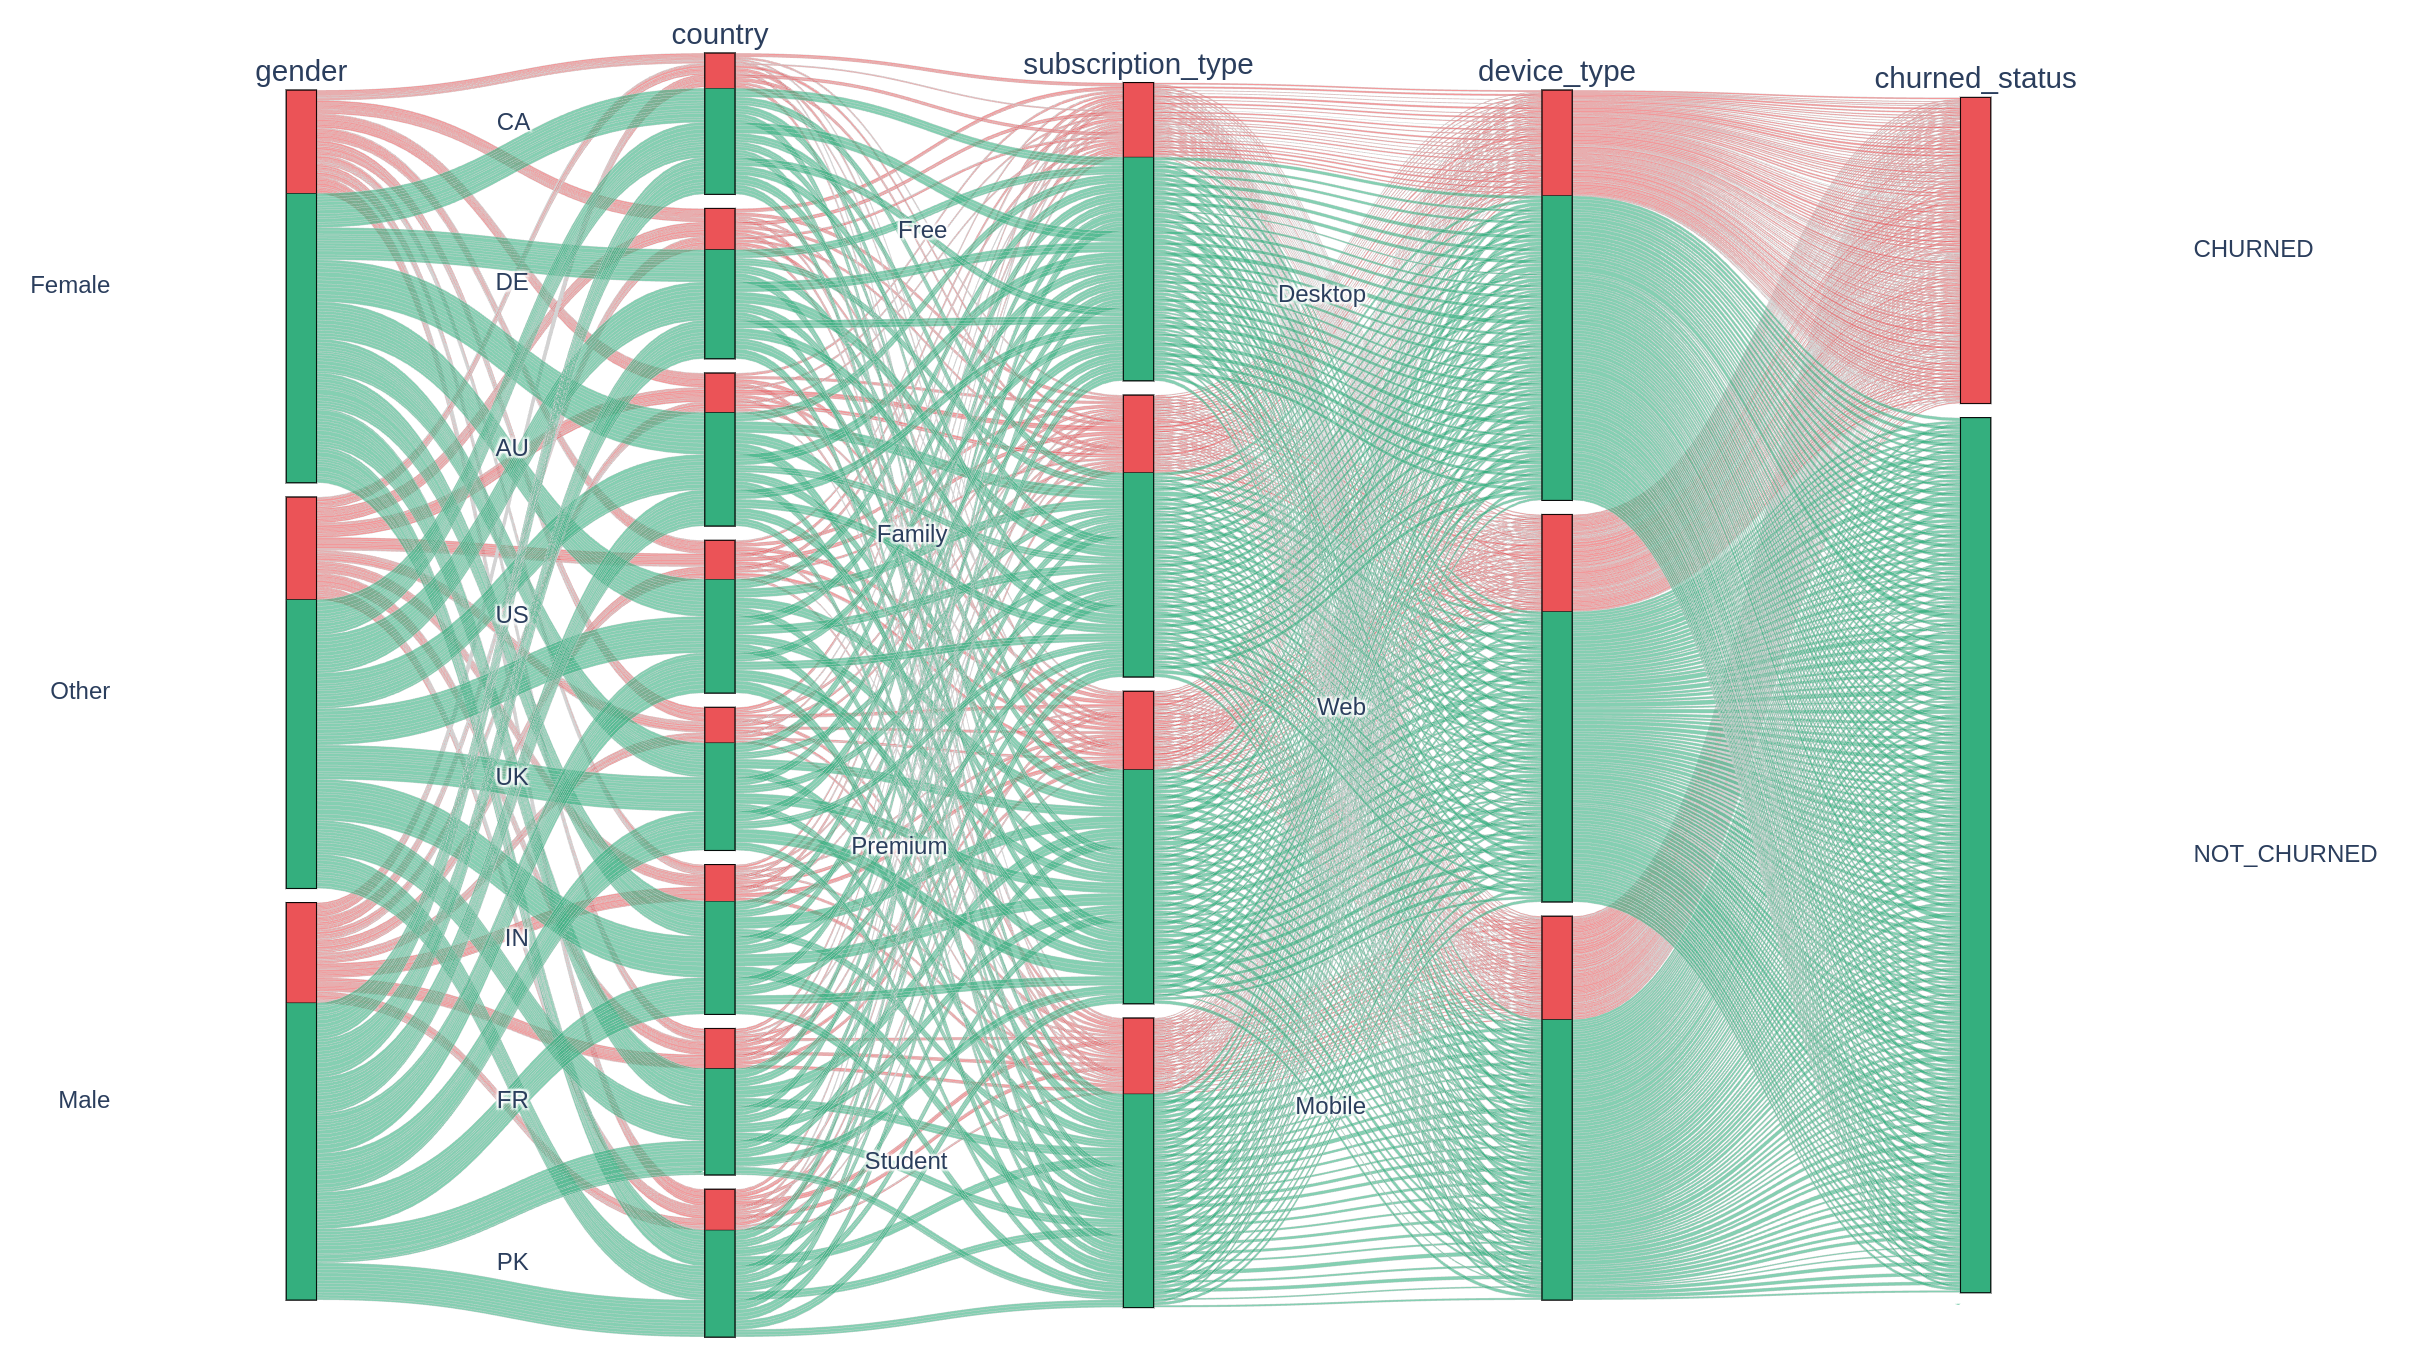
\includegraphics[width=1.0\textwidth, keepaspectratio]{secciones/sec2/imagenes/churn_spotify_ParallelCategories_NominalAttributes.png}}
    \caption{Visualización de categorías paralelas en las variables categóricas.}
    \label{fig:churn_spotify_ParallelCategories_NominalAttributes}
\end{figure} 

Esto coincide con el análisis estadístico presentado en la Figura \ref{}, en el que en ningún caso se puede rechazar ---con un 95\% de confianza--- la hipótesis nula de independencia entre variables categóricas (\textit{p-values} superiores al 5\%), ya sea entre atributos o entre cada atributo y la variable objetivo.

\begin{tcolorbox}
    [colback=gray!5!white, colframe=gray!60!black, title=Correlación entre dos variables categóricas]

    Se emplea Test Chi Cuadrado...  
    Cuando se rechaza la hipótesis nula (\textit{p-value}$<0.05$) y, por tanto, que las variables sean independientes, el Test V de Cramer permite medir el impacto de la asociación entre ambas variables.

\end{tcolorbox}

El análisis de ... 


\paragraph*{Variables numéricas.}

%Primero, analizamos cada variable numérica individualmente. ¿Qué valores abarca? ¿Media/Mediana?
% Comentar la variable offline_listening que es binaria


%Segundo, ¿cómo se correlacionan unas con otras?
En la Figura \ref{} podemos ver una matriz de correlación entre las variables numéricas. Las únicas correlaciones significativas la encontramos entre \code{offline\_listening} y \code{ads\_listened\_per\_week}, que se correlacionan inversamente, cosa que tiene sentido porque solo pueden usar el modo \textit{offline} aquellos usuarios con cuenta \textit{premium} (ya sea la básica, familiar o de estudiante), que son los usuarios a los que no se les reproduce anuncios.

\begin{tcolorbox}
    [colback=gray!5!white, colframe=gray!60!black, title=Medida de asociación]

    Para analizar la asociación entre una variable numérica y una variable categórica se realiza comparación de distribuciones de la variable numérica entre los diferentes grupos definidos por la variable categórica.

    Hay varias pruebas estadísticas:
    \begin{itemize}
        \item \textbf{Pruebas paramétricas}: Estas pruebas asumen que la variable numérica sigue una distribución específica (generalmente la normal).
        
        Las siguientes pruebas asumen que la variable numérica sigue una distribución normal en cada grupo y que las varianzas de los grupos son aproximadamente iguales (homocedasticidad).

        \begin{itemize}
            \item Prueba $t$ de Student: Para dos grupos. ...
            \item Análisis de varianza (ANOVA): Para tres o más grupos. ...
        \end{itemize}

        También encontramos pruebas diseñadas para casos en los que la variable numérica presenta normalidad pero no homocedasticidad:

        \begin{itemize}
            \item Prueba $t$ de Welch: Para dos grupos. ...
            \item Pruba Welch ANOVA: Para tres o más grupos. ...
        \end{itemize}
        
        \item \textbf{Pruebas no parámetricas}: Estas pruebas se utilizan en casos en los que las variables no se ajustan a modelos teóricos. Estas pruebas son menos efectivas que las parámetricas para distribuciones normales, pero en los casos en los que no se cumplen los supuestos paramétricos (como normalidad), son más robustas y fiables. Se basan en los rangos de los datos.
        
        Algunas de estas pruebas son:
        
        \begin{itemize}
            \item Prueba $U$ de Mann-Whitney: Alternativa a la prueba $t$ de Student que compara las medianas o distribuciones de los rangos de dos grupos independientes.
            \item Prueba de Kruskal-Wallis: Alternativa al ANOVA que compara las medianas o distribuciones de los rangos de tres o más grupos independientes.
        \end{itemize}
        
        Cuando se comparan tres o más grupos, si la prueba ANOVA, Welch ANOVA o de Kruskal-Wallis resulta significativa, generalmente se requieren pruebas \textit{post-hoc} (como la prueba de Tukey para ANOVA, prueba \textit{post-hoc} de Games-Howell comparaciones por pares de Mann-Whitney con corrección de Bonferroni) para determinar cuáles grupos difieren entre sí.
        
    \end{itemize}
    
\end{tcolorbox}

%¿Cómo se relacionan las variables con la variable objetivo?





\subsubsection{Codificación de las variables categóricas}


\subsubsection{Normalización de las variables numéricas}

